Se asume que los casos de uso en los que interviene el \textbf{rol de comercial} pueden ser igualmente realizados por el \textbf{rol de administrador}, al disponer este de permisos equivalentes o superiores dentro del sistema. Por este motivo, y con el objetivo de mejorar la \textbf{claridad del modelo}, se ha optado por representar únicamente el rol de comercial en algunos casos de uso compartidos, evitando redundancias innecesarias en los diagramas. No obstante, en aquellos casos en los que existen \textbf{funcionalidades exclusivas del rol de administrador}, este se ha representado explícitamente.

Este enfoque es coherente con el \textbf{modelado de casos de uso}, en el que los actores representan roles que interactúan con el sistema \citep[Ch.~4]{sommerville}.

\bigskip

Los diagramas se han organizado siguiendo la \textbf{división modular} definida en la Sección~\ref{sec:ModularRequirements}:

\begin{itemize}
    \item \texttt{M1}: recoge los casos de uso de \textbf{acceso, sesiones, perfil y administración de cuentas}.
    \item \texttt{M2}: agrupa la \textbf{gestión comercial}, la planificación de visitas, rutas, estimaciones de llegada y avisos asociados.
    \item \texttt{M3}: representa las operaciones sobre \textbf{catálogo, productos, información técnica y coloración}.
    \item \texttt{M4}: diferencia \textbf{pedido, método de entrega, preparación de repartos, etiquetas, validación de entrega y cobros}.
    \item \texttt{M5}: recoge la \textbf{gestión técnica del salón}, incluyendo fichas, servicios, historial, plantillas, imágenes, sugerencias y borradores técnicos.
    \item \texttt{M6}: concentra \textbf{promociones, rangos, notificaciones, canales externos y formaciones}.
    \item \texttt{M7}: se reserva para la \textbf{administración transversal del sistema}.
    \item \texttt{M8}: se mantiene como módulo de \textbf{funcionalidades adicionales} y \textbf{trabajo futuro}.
\end{itemize}

\newpage{\ }
\subsection{Casos de Uso M1.}

La Figura~\ref{fig:M1_CasosDeUso} representa los casos de uso relacionados con la \textbf{gestión de acceso, alta y autorización de usuarios}.

\begin{figure}[H]
    \centering
    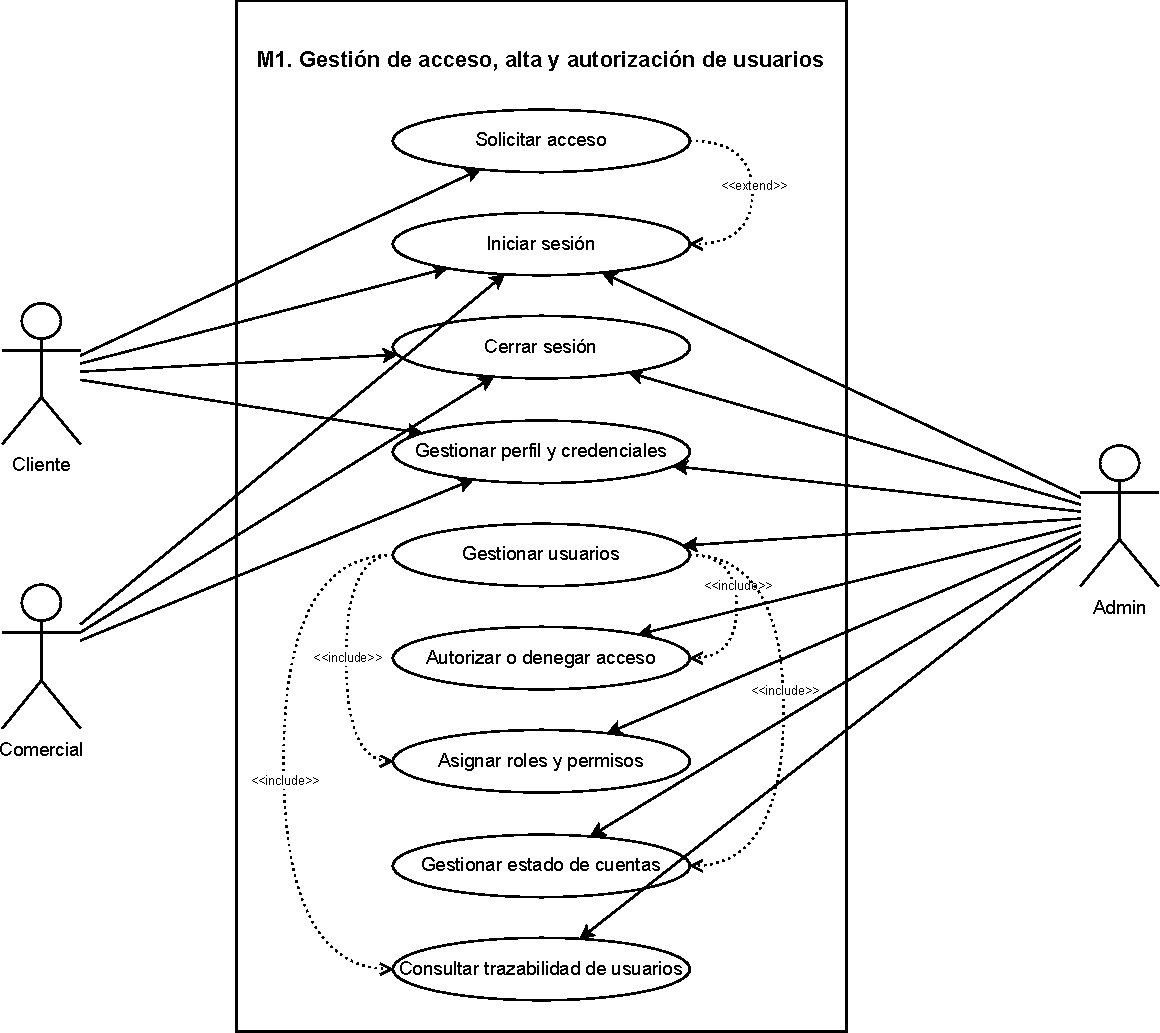
\includegraphics[width=\textwidth,height=0.72\textheight,keepaspectratio]{./figures/UML/CasosDeUso/M1_CasosDeUso.pdf}
    \caption{Casos de Uso M1. Gestión de acceso, alta y autorización de usuarios}
    \label{fig:M1_CasosDeUso}
\end{figure}

\newpage{\ }
\subsection{Casos de Uso M2.}

La Figura~\ref{fig:M2_CasosDeUso} representa los casos de uso relacionados con la \textbf{gestión comercial}, los \textbf{clientes profesionales}, la planificación de visitas y el soporte a rutas.

\begin{figure}[H]
    \centering
    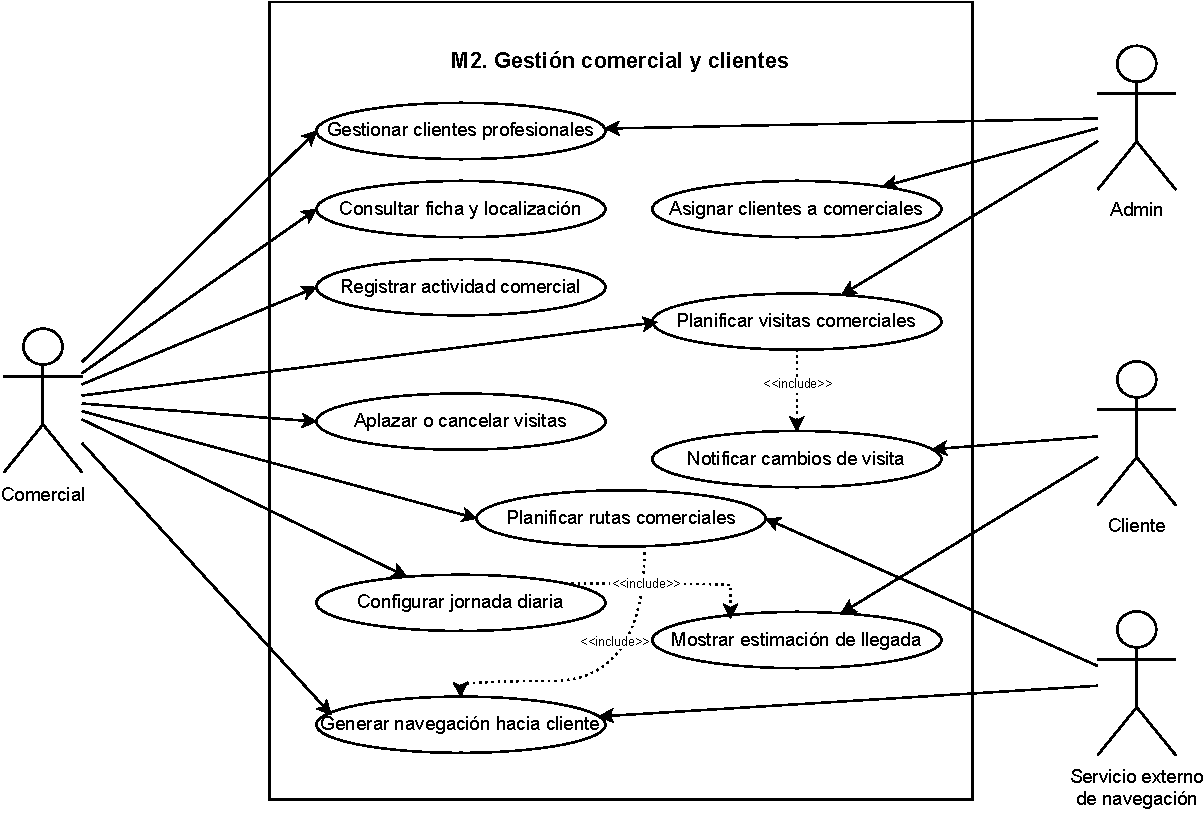
\includegraphics[width=\textwidth,height=0.72\textheight,keepaspectratio]{./figures/UML/CasosDeUso/M2_CasosDeUso.pdf}
    \caption{Casos de Uso M2. Gestión comercial y clientes}
    \label{fig:M2_CasosDeUso}
\end{figure}

\newpage{\ }
\subsection{Casos de Uso M3.}

La Figura~\ref{fig:M3_CasosDeUso} representa los casos de uso relacionados con el \textbf{catálogo}, los \textbf{productos} y la \textbf{coloración}.

\begin{figure}[H]
    \centering
    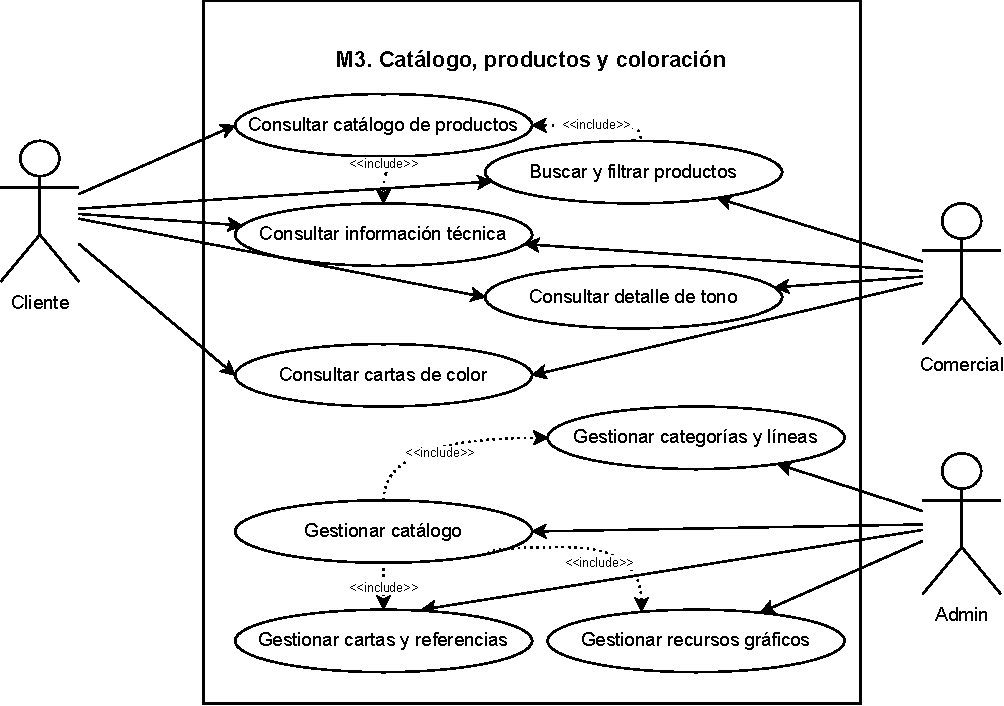
\includegraphics[width=\textwidth,height=0.72\textheight,keepaspectratio]{./figures/UML/CasosDeUso/M3_CasosDeUso.pdf}
    \caption{Casos de Uso M3. Catálogo, productos y coloración}
    \label{fig:M3_CasosDeUso}
\end{figure}

\newpage{\ }
\subsection{Casos de Uso M4.}

La Figura~\ref{fig:M4_CasosDeUso} representa los casos de uso relacionados con los \textbf{pedidos}, la \textbf{preparación de repartos}, las entregas por comercial o agencia, la \textbf{trazabilidad} y los cobros parciales o totales.

\begin{figure}[H]
    \centering
    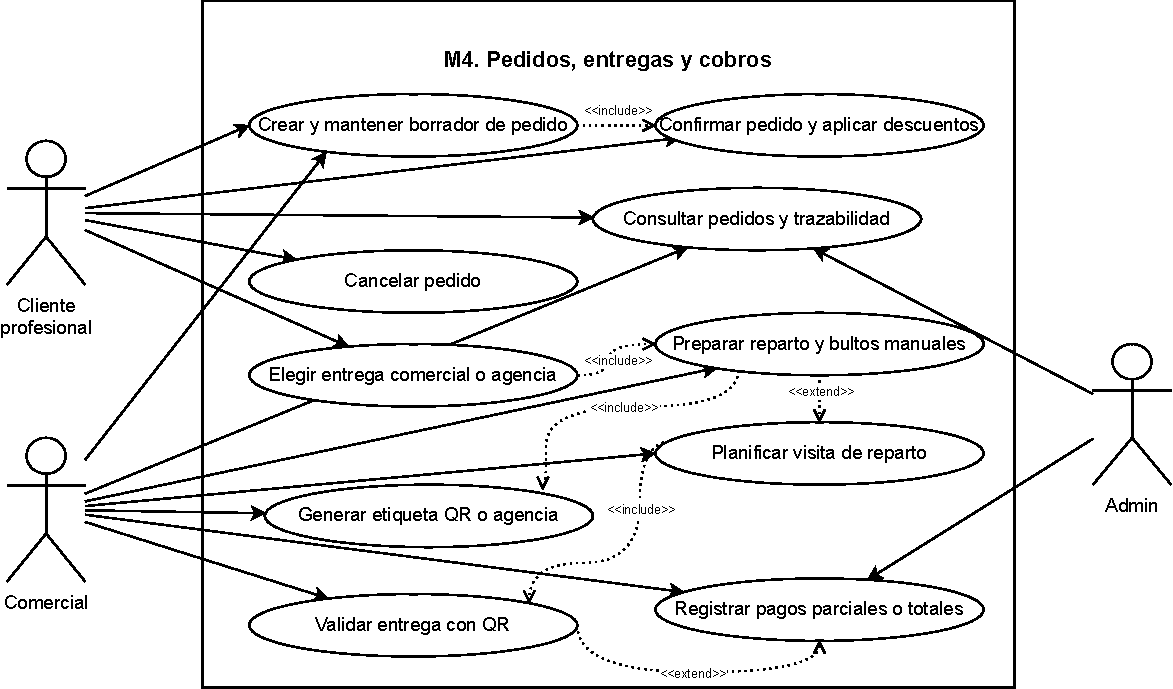
\includegraphics[width=\textwidth,height=0.72\textheight,keepaspectratio]{./figures/UML/CasosDeUso/M4_CasosDeUso.pdf}
    \caption{Casos de Uso M4. Pedidos, entregas y cobros}
    \label{fig:M4_CasosDeUso}
\end{figure}

\newpage{\ }
\subsection{Casos de Uso M5.}

La Figura~\ref{fig:M5_CasosDeUso} representa los casos de uso relacionados con la \textbf{gestión técnica interna de los salones}: fichas de clientes, servicios realizados, fichas técnicas, historial, productos utilizados, plantillas reutilizables, imágenes de resultado, sugerencias derivadas y preparación de borradores técnicos.

\begin{figure}[H]
    \centering
    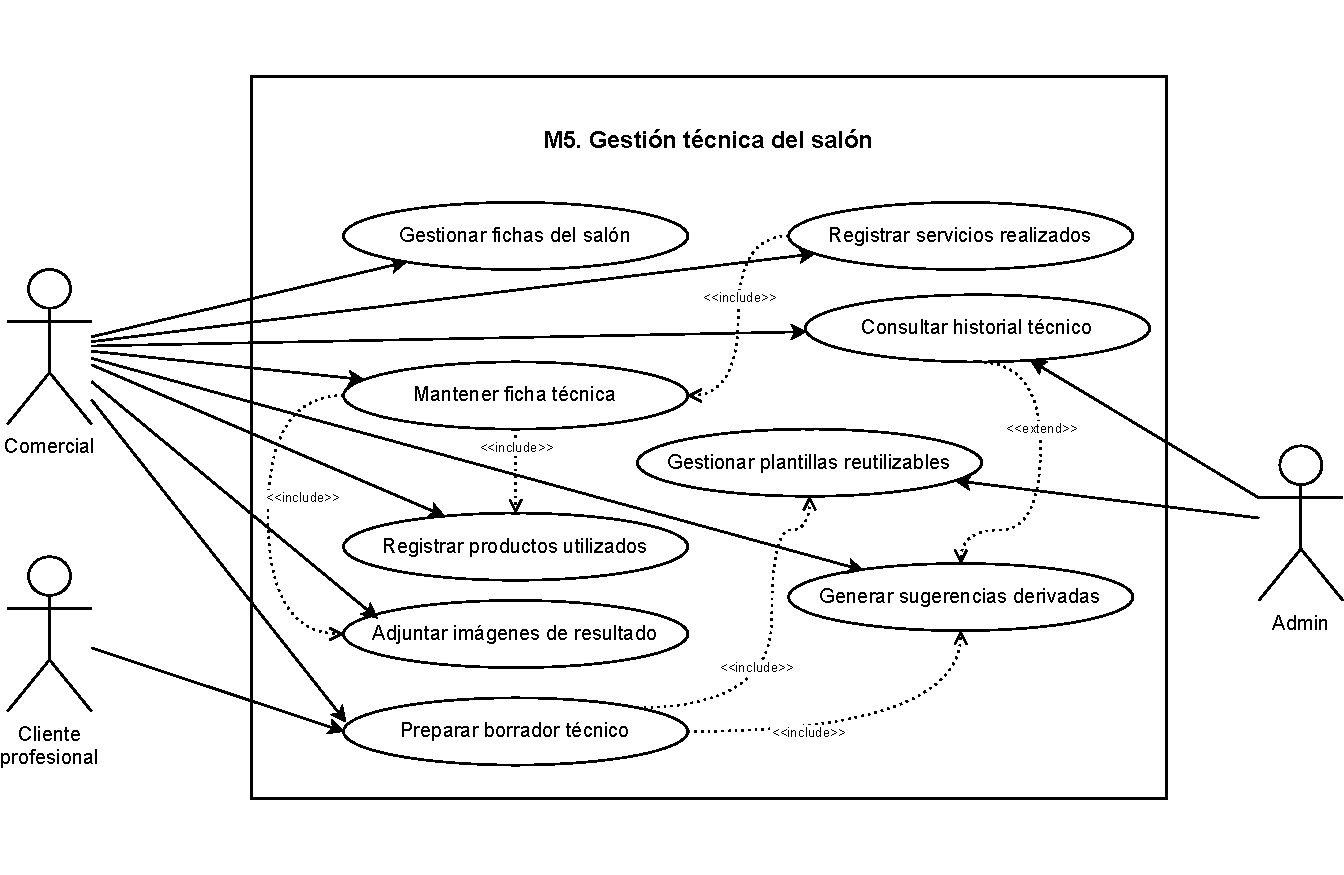
\includegraphics[width=\textwidth,height=0.72\textheight,keepaspectratio]{./figures/UML/CasosDeUso/M5_CasosDeUso.pdf}
    \caption{Casos de Uso M5. Gestión técnica del salón}
    \label{fig:M5_CasosDeUso}
\end{figure}

\newpage{\ }
\subsection{Casos de Uso M6.}

La Figura~\ref{fig:M6_CasosDeUso} representa los casos de uso relacionados con \textbf{promociones}, \textbf{rangos comerciales}, notificaciones, comunicaciones por canales externos y formaciones. Las promociones se conectan con la consulta por parte de clientes y comerciales, con la aplicación de descuentos en pedidos y con la gestión administrativa de segmentos, adjuntos, recordatorios e inscripciones.

\begin{figure}[H]
    \centering
    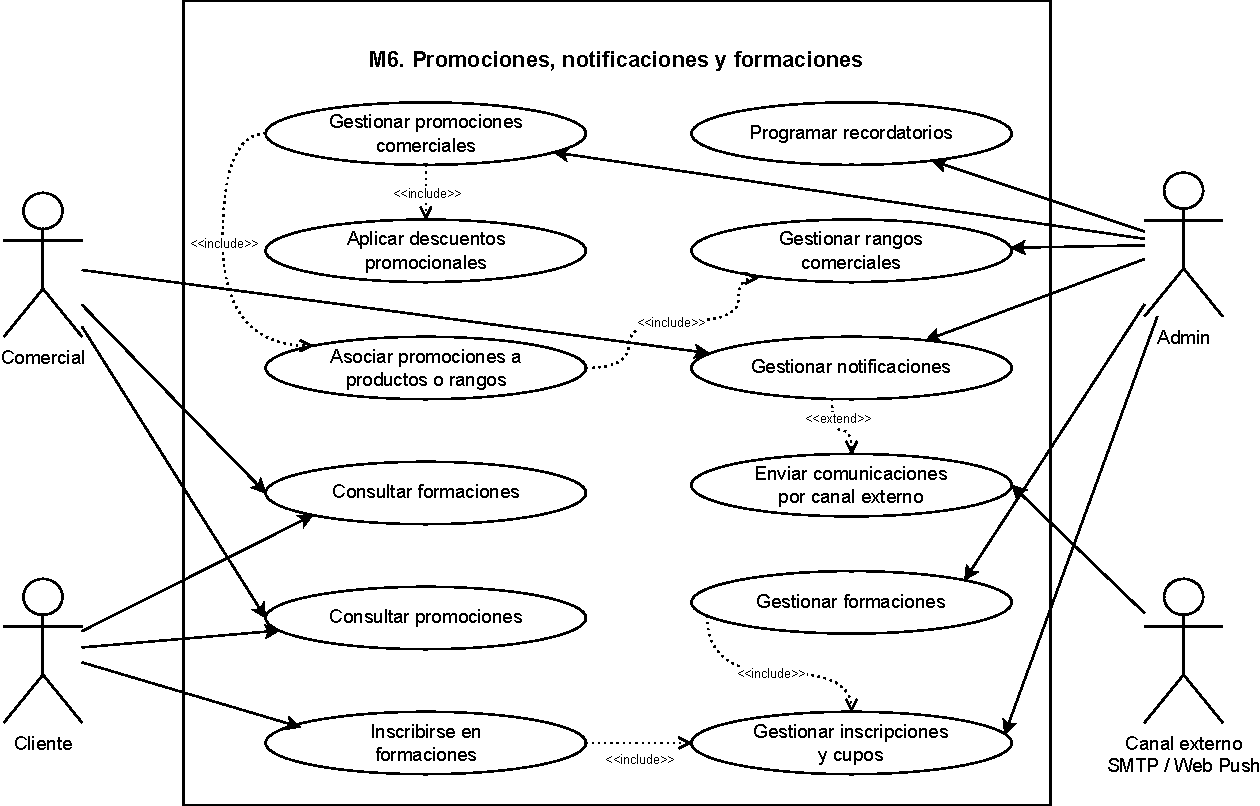
\includegraphics[width=\textwidth,height=0.72\textheight,keepaspectratio]{./figures/UML/CasosDeUso/M6_CasosDeUso.pdf}
    \caption{Casos de Uso M6. Promociones, notificaciones y formaciones}
    \label{fig:M6_CasosDeUso}
\end{figure}

\newpage{\ }
\subsection{Casos de Uso M7.}

La Figura~\ref{fig:M7_CasosDeUso} representa los casos de uso relacionados con la \textbf{administración transversal del sistema}: configuración común, canales de aviso, cargo por agencia, umbrales de rangos, auditoría, propuestas internas de pedido a proveedor, servicios auxiliares, diagnóstico técnico de \textit{rate limiting} y soporte de compatibilidad o instalación \textit{PWA} \citep{webdev-pwa}.

\begin{figure}[H]
    \centering
    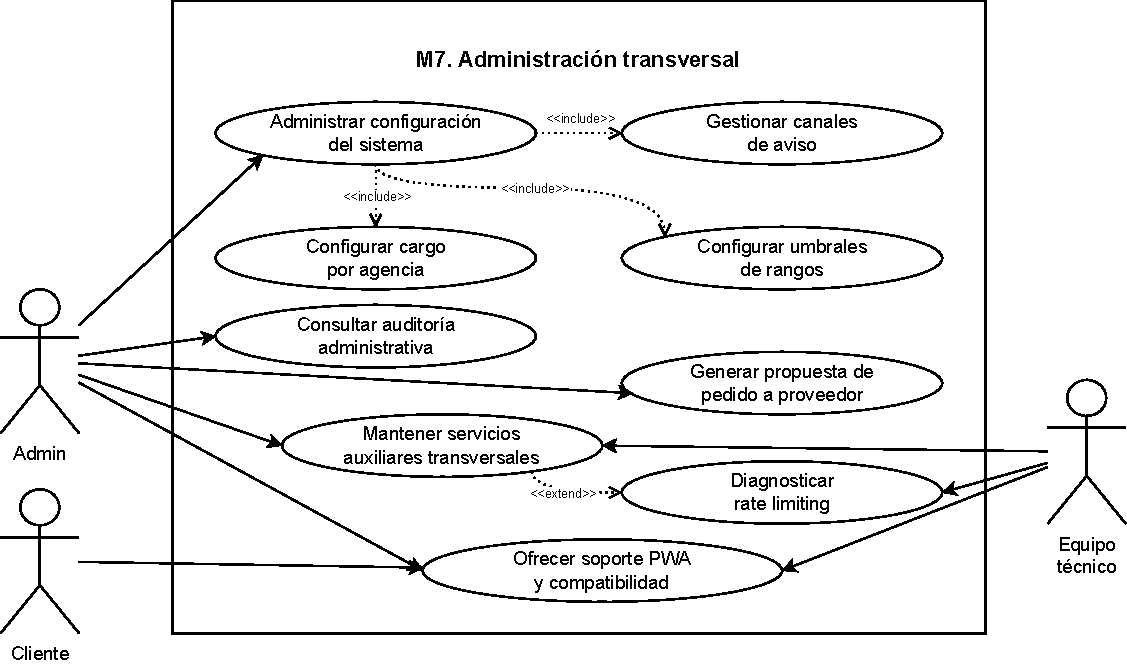
\includegraphics[width=\textwidth,height=0.72\textheight,keepaspectratio]{./figures/UML/CasosDeUso/M7_CasosDeUso.pdf}
    \caption{Casos de Uso M7. Administración transversal}
    \label{fig:M7_CasosDeUso}
\end{figure}

\newpage{\ }
\subsection{Casos de Uso M8.}

La Figura~\ref{fig:M8_CasosDeUso} representa los casos de uso relacionados con \textbf{funcionalidades adicionales} y \textbf{trabajo futuro}. Este módulo agrupa capacidades avanzadas que no forman parte del alcance principal de la versión actualmente implementada: \textbf{diagnóstico capilar con capilógrafo} e inteligencia artificial, simulación de estilos o coloración mediante cámara móvil, reconocimiento de productos, reserva \textit{online}, asistente virtual tipo \textit{chatbot} y automatización de servicios externos como Factusol mediante flujos con \textit{n8n} o \textit{APIs} equivalentes \citep{sdelsol-factusol,n8n-webhook,n8n-http-request}.

\begin{figure}[H]
    \centering
    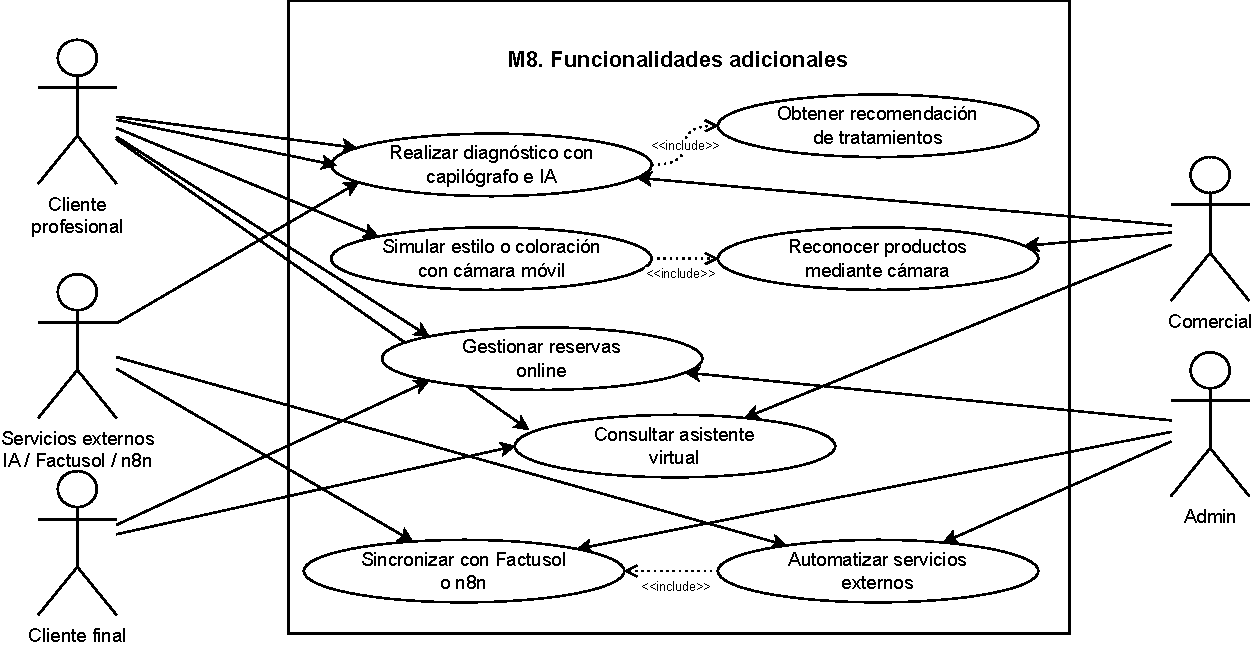
\includegraphics[width=\textwidth,height=0.72\textheight,keepaspectratio]{./figures/UML/CasosDeUso/M8_CasosDeUso.pdf}
    \caption{Casos de Uso M8. Funcionalidades adicionales}
    \label{fig:M8_CasosDeUso}
\end{figure}
